% Lines that start with a % are comments and are not included when the LaTeX file is converted to a pdf

% Set up the document class - this can be changed if a different format is required 
\documentclass[12pt,a4paper]{article}
\usepackage[utf8]{inputenc}
\usepackage{amsmath}
\usepackage{amsfonts}
\usepackage{amssymb}
\usepackage{graphicx}
\usepackage{url}
\usepackage{hyperref}
\usepackage[left=2cm,right=2cm,top=2cm,bottom=2cm]{geometry}


% Include packages that contain additional features, for example including special mathematical characters and images in your document
\usepackage{enumitem}
\usepackage{pdfpages}
% The beginning of the document...
\begin{document}

% Please change the following accordingly...
\centerline{\large Exercises sheet 8}\vspace{0.5em}
\centerline{\large by Maximilian Richter and Christian Heppe}\vspace{2em}

% Split the different exercises into different sections...
\section*{Exercise 2: Lorenz-attractor}
\subsection*{1.}
As one can see in Figure 1, starting near a fixed point with values of $r<24$, the trajectory of the system stays quite stable and shows a pretty "linear" path converging into the attractor.\\
\newline
Starting near a fixed point with value $r\ge 24$, the system starts to do an oscillation-like movement around the fixed point and for $r=28$ it does it with a deterministic chaotic behaviour to flip side into a second plane, but it can't be determined when exactly the system changes the plane. This means the movement of the system is chaotic. The trajectories of the system follow a strange attractor and it seems to be one of the most simple chaotic systems. For further illustration of the movement see the GIF file in the following link (file was too big for e-mail attachement, unfortunately you have to download it in order to see it)\\
\url{https://www.dropbox.com/s/82l1riodcpra9a4/lorenz_attractor_tiny.gif?dl=0} .\\
\newline
The variable $r$ is a parameter which changes the behaviour of a system dramatically at a critical value. It can be identified with the Rayleigh-Number, which characterizes the flow of a fluid under thermal influence. If the number is blow a critical value it shows "laminar" behaviour comparable with thermal conduction. If the number is above a critical value (here in this system its $24>r>28$) the system flow is comparable to thermal convection of a heated fluid and show turbulences and chaotic movements. 
\subsection*{2.}
In Figure 2 one can see the local minima $z_{k+1}$ as a function of $z_k$. The minima-function should have a slope $|m|>1$ in order to be periodic. As one can see in Figure 2, the interpolation of the points with a linear fit yields that the local minima and hence the lorenz-attractor \textbf{does} have a slope $|m|>1$ for $r=27$. 
\begin{align*}
	m=1.0427
\end{align*}
This means the oscillator-like movement and thus the Lorenz-attractor is in fact \textbf{not} a periodic movement. 
\begin{figure}[h]
\centering
	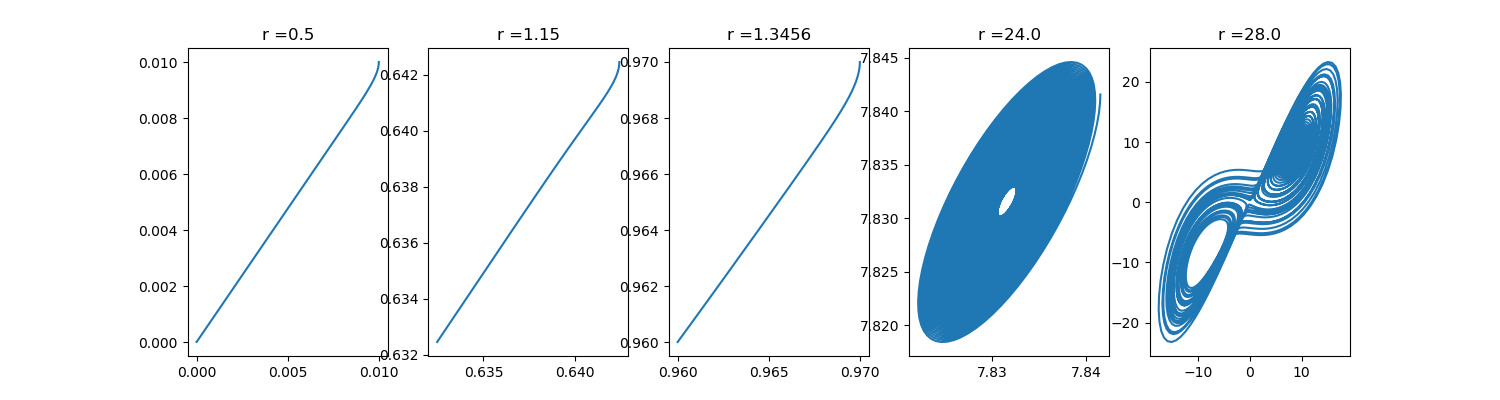
\includegraphics[width=1\textwidth]{lorenz.png}
	\caption{Lorenz-attractor for different values of $r$}
\end{figure}
\begin{figure}[h]
\centering
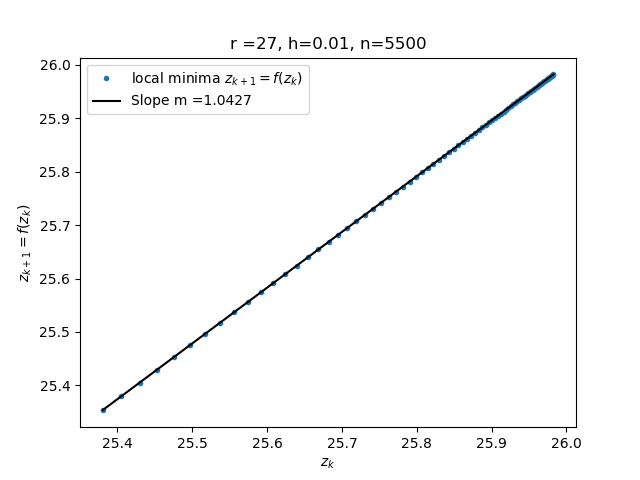
\includegraphics[width=0.7\textwidth]{lorenzz.png}
\caption{Local minima $z_{k+1}$ as a function of $z_k$}
\end{figure}

\end{document}
